\documentclass[tikz,border=8pt]{standalone}
\usepackage{tikz}
\usetikzlibrary{positioning,fit,arrows.meta,calc,backgrounds,shadows}

\definecolor{encBlue}{HTML}{1F77B4}
\definecolor{decOrange}{HTML}{FF7F0E}
\definecolor{outGreen}{HTML}{2CA02C}
\definecolor{memPurple}{HTML}{9467BD}
\definecolor{maskRed}{HTML}{D62728}
\definecolor{textDark}{HTML}{111827}
\definecolor{panelBlue}{HTML}{EAF3FB}
\definecolor{panelOrange}{HTML}{FFF0DF}
\definecolor{panelGreen}{HTML}{EAF7EF}

\begin{document}
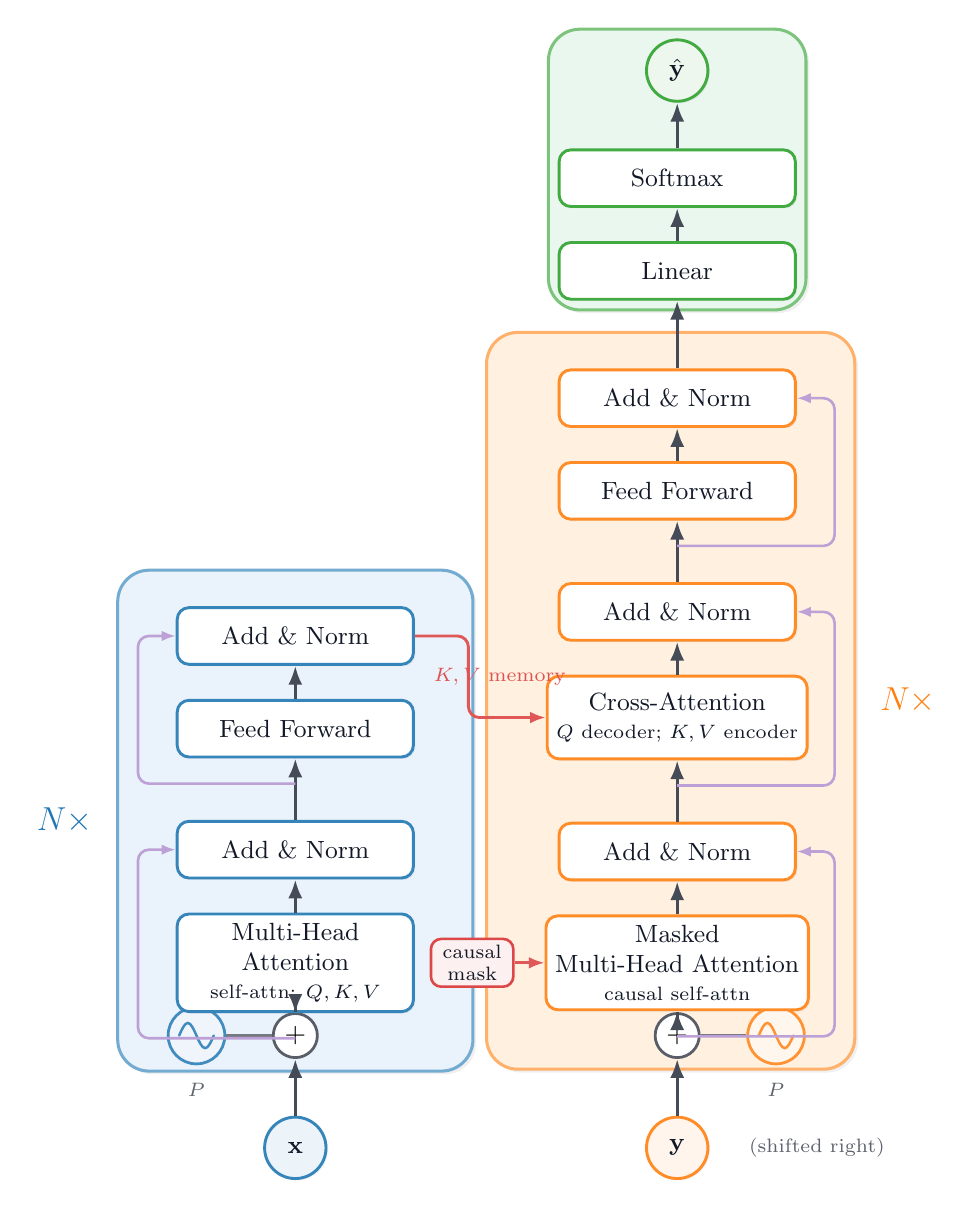
\begin{tikzpicture}[
  >=Latex,
  main/.style={-{Latex[length=2.4mm]}, line width=1.2pt, draw=textDark!78},
  residual/.style={-{Latex[length=1.8mm]}, line width=0.95pt, rounded corners=4pt, draw=memPurple!62},
  memory/.style={-{Latex[length=2.0mm]}, line width=1.05pt, rounded corners=4pt, draw=maskRed!78},
  panel/.style={
    rectangle,
    rounded corners=4mm,
    draw=#1!62,
    fill=#1!8,
    line width=1.1pt,
    drop shadow={shadow xshift=1.2pt, shadow yshift=-1.2pt, opacity=0.12}
  },
  layer/.style={
    rectangle,
    rounded corners=1.5mm,
    draw=#1!90,
    fill=white,
    line width=1.05pt,
    minimum width=3.0cm,
    minimum height=0.72cm,
    align=center,
    font=\small,
    text=textDark,
    drop shadow={shadow xshift=0.7pt, shadow yshift=-0.7pt, opacity=0.10}
  },
  tall layer/.style={layer=#1, minimum height=1.05cm},
  token/.style={
    circle,
    draw=#1!90,
    fill=#1!8,
    line width=1.05pt,
    minimum size=0.78cm,
    font=\small\bfseries,
    text=textDark,
    drop shadow={shadow xshift=0.7pt, shadow yshift=-0.7pt, opacity=0.10}
  },
  sum/.style={
    circle,
    draw=textDark!70,
    fill=white,
    line width=1.0pt,
    minimum size=0.56cm,
    inner sep=0pt,
    font=\bfseries
  },
  tag/.style={
    rectangle,
    rounded corners=1.3mm,
    draw=#1!85,
    fill=#1!7,
    line width=0.95pt,
    align=center,
    font=\scriptsize,
    text=textDark,
    inner xsep=0.42em,
    inner ysep=0.22em
  },
  pe/.style={
    circle,
    draw=#1!85,
    fill=#1!7,
    line width=1.0pt,
    minimum size=0.72cm,
    path picture={
      \draw[#1!85, line width=0.9pt, line cap=round]
        ([xshift=-0.22cm]path picture bounding box.center)
        sin ++(0.11cm,0.16cm) cos ++(0.11cm,-0.16cm)
        sin ++(0.11cm,-0.16cm) cos ++(0.11cm,0.16cm);
    }
  },
  note/.style={font=\scriptsize, text=textDark!68}
]
  % Inputs
  \node[token=encBlue] (x) at (0,0) {$\mathbf{x}$};
  \node[token=decOrange] (y) at (4.85,0) {$\mathbf{y}$};
  \node[sum, above=0.72cm of x] (xsum) {$+$};
  \node[sum, above=0.72cm of y] (ysum) {$+$};
  \node[pe=encBlue, left=0.58cm of xsum] (xpos) {};
  \node[pe=decOrange, right=0.58cm of ysum] (ypos) {};
  \node[note, below=0.10cm of xpos] {$P$};
  \node[note, below=0.10cm of ypos] {$P$};
  \node[note, right=0.38cm of y] {(shifted right)};

  % Encoder
  \node[tall layer=encBlue] (encAttn) at (0,2.35)
    {Multi-Head\\Attention\\[-1pt]{\scriptsize self-attn: $Q,K,V$}};
  \node[layer=encBlue, above=0.42cm of encAttn] (encNorm1) {Add \& Norm};
  \node[layer=encBlue, above=0.78cm of encNorm1] (encFFN) {Feed Forward};
  \node[layer=encBlue, above=0.42cm of encFFN] (encNorm2) {Add \& Norm};

  % Decoder
  \node[tall layer=decOrange] (decMasked) at (4.85,2.35)
    {Masked\\Multi-Head Attention\\[-1pt]{\scriptsize causal self-attn}};
  \node[layer=decOrange, above=0.42cm of decMasked] (decNorm1) {Add \& Norm};
  \node[tall layer=decOrange, above=0.78cm of decNorm1] (decCross)
    {Cross-Attention\\[-1pt]{\scriptsize $Q$ decoder; $K,V$ encoder}};
  \node[layer=decOrange, above=0.42cm of decCross] (decNorm2) {Add \& Norm};
  \node[layer=decOrange, above=0.78cm of decNorm2] (decFFN) {Feed Forward};
  \node[layer=decOrange, above=0.42cm of decFFN] (decNorm3) {Add \& Norm};

  % Output head
  \node[layer=outGreen, above=0.86cm of decNorm3] (linear) {Linear};
  \node[layer=outGreen, above=0.42cm of linear] (softmax) {Softmax};
  \node[token=outGreen, above=0.58cm of softmax] (yhat) {$\hat{\mathbf{y}}$};

  % Main flows
  \draw[main] (x) -- (xsum);
  \draw[main] (xsum) -- (encAttn);
  \draw[main] (encAttn) -- (encNorm1);
  \draw[main] (encNorm1) -- (encFFN);
  \draw[main] (encFFN) -- (encNorm2);

  \draw[main] (y) -- (ysum);
  \draw[main] (ysum) -- (decMasked);
  \draw[main] (decMasked) -- (decNorm1);
  \draw[main] (decNorm1) -- (decCross);
  \draw[main] (decCross) -- (decNorm2);
  \draw[main] (decNorm2) -- (decFFN);
  \draw[main] (decFFN) -- (decNorm3);
  \draw[main] (decNorm3) -- (linear);
  \draw[main] (linear) -- (softmax);
  \draw[main] (softmax) -- (yhat);

  \draw[textDark!58, line width=0.9pt] (xpos) -- (xsum);
  \draw[textDark!58, line width=0.9pt] (ypos) -- (ysum);

  % Residual paths, kept light and outside the main vertical spine.
  \draw[residual] ($(encAttn.south)+(0,-0.32)$) -| ($(encNorm1.west)+(-0.48,-0.30)$) |- (encNorm1.west);
  \draw[residual] ($(encFFN.south)+(0,-0.32)$) -| ($(encNorm2.west)+(-0.48,-0.30)$) |- (encNorm2.west);
  \draw[residual] ($(decMasked.south)+(0,-0.32)$) -| ($(decNorm1.east)+(0.48,-0.30)$) |- (decNorm1.east);
  \draw[residual] ($(decCross.south)+(0,-0.32)$) -| ($(decNorm2.east)+(0.48,-0.30)$) |- (decNorm2.east);
  \draw[residual] ($(decFFN.south)+(0,-0.32)$) -| ($(decNorm3.east)+(0.48,-0.30)$) |- (decNorm3.east);

  % Causal mask and encoder memory are the only non-main semantic arrows.
  \node[tag=maskRed, left=0.38cm of decMasked] (mask) {causal\\mask};
  \draw[memory] (mask) -- (decMasked);
  \draw[memory] (encNorm2.east) -- ++(0.68,0) |- (decCross.west);
  \node[note, text=maskRed!80] at ($(encNorm2.east)+(1.08,-0.52)$) {$K,V$ memory};

  % Background panels
  \coordinate (encSW) at ($(encAttn.south west)+(-0.62,-0.62)$);
  \coordinate (encNE) at ($(encNorm2.north east)+(0.62,0.34)$);
  \coordinate (decSW) at ($(decMasked.south west)+(-0.62,-0.62)$);
  \coordinate (decNE) at ($(decNorm3.north east)+(0.62,0.34)$);
  \begin{scope}[on background layer]
    \node[panel=encBlue, fill=panelBlue, fit=(encSW)(encNE)] (encoder) {};
    \node[panel=decOrange, fill=panelOrange, fit=(decSW)(decNE)] (decoder) {};
    \node[panel=outGreen, fill=panelGreen, fit=(linear)(softmax)(yhat)] {};
  \end{scope}

  \node[font=\large\bfseries, text=encBlue, anchor=east] at ($(encoder.west)+(-0.18,0)$) {$N\times$};
  \node[font=\large\bfseries, text=decOrange, anchor=west] at ($(decoder.east)+(0.18,0)$) {$N\times$};
\end{tikzpicture}
\end{document}
